%----------------------------------------------------------------------------
\appendix
%----------------------------------------------------------------------------
\chapter*{\fuggelek}\addcontentsline{toc}{chapter}{\fuggelek}
\setcounter{chapter}{\appendixnumber}
%\setcounter{equation}{0} % a fofejezet-szamlalo az angol ABC 6. betuje (F) lesz
\numberwithin{equation}{section}
\numberwithin{figure}{section}
\numberwithin{lstlisting}{section}
%\numberwithin{tabular}{section}

\section{Teszteredmények}
\label{sec:fug_teszt_ered}

\begin{figure}[ht] 
	\begin{subfigure}[b]{0.5\linewidth}
		\centering
		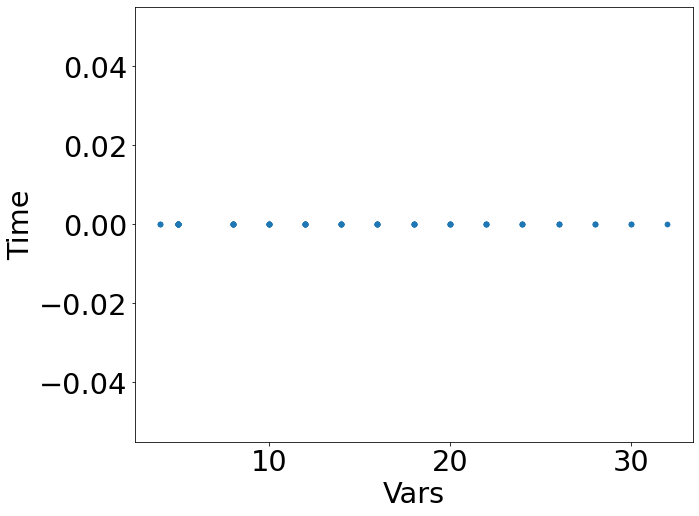
\includegraphics[width=0.95\linewidth]{figures/locks/vars.png} 
		\caption{Változók} 
		\vspace{4ex}
	\end{subfigure}%% 
	\begin{subfigure}[b]{0.5\linewidth}
		\centering
		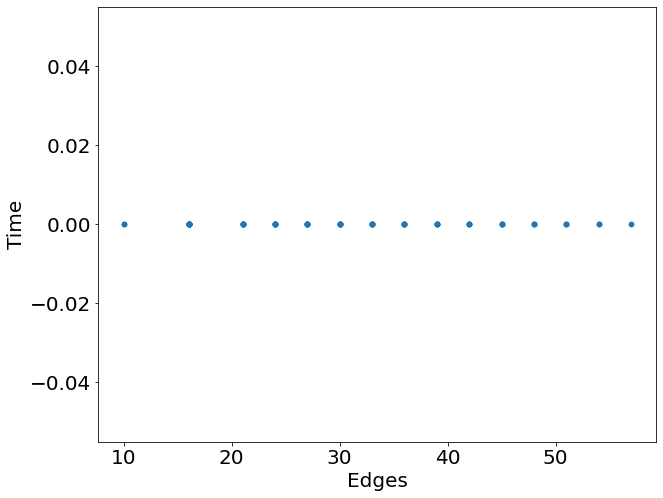
\includegraphics[width=0.95\linewidth]{figures/locks/edges.png} 
		\caption{Élek} 
		\vspace{4ex}
	\end{subfigure} 
	\begin{subfigure}[b]{0.5\linewidth}
		\centering
		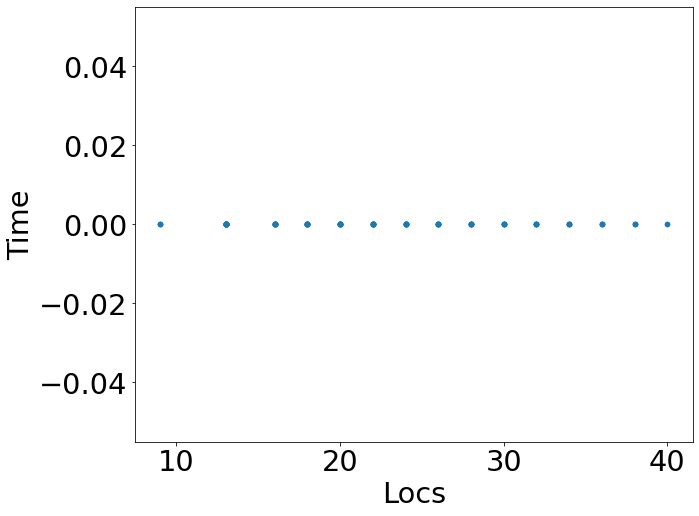
\includegraphics[width=0.95\linewidth]{figures/locks/locs.png} 
		\caption{Helyek} 
	\end{subfigure}%%
	\begin{subfigure}[b]{0.5\linewidth}
		\centering
		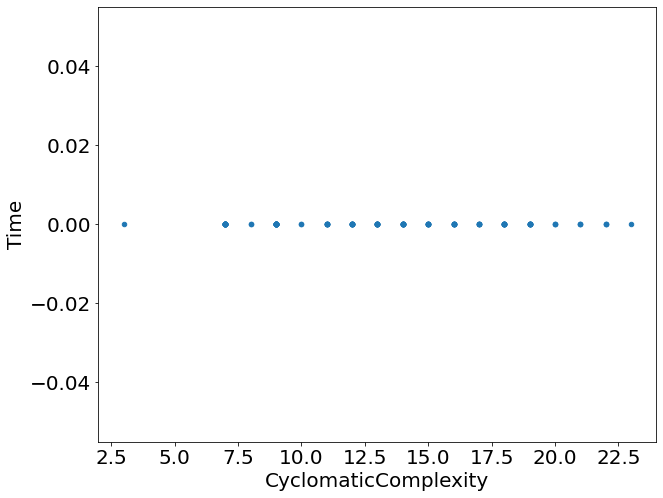
\includegraphics[width=0.95\linewidth]{figures/locks/cc.png} 
		\caption{Ciklikus komplexitás} 
	\end{subfigure} 
	\caption{Locks tesztkategória.\label{fig:locks} }
\end{figure}

\begin{figure}[ht] 
	\begin{subfigure}[b]{0.5\linewidth}
		\centering
		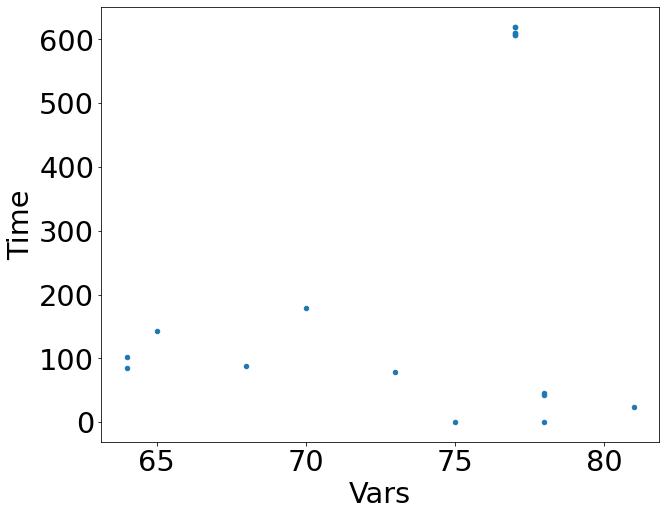
\includegraphics[width=0.95\linewidth]{figures/ssh/vars.png} 
		\caption{Változók\label{fig_ssh_a}} 
		\vspace{4ex}
	\end{subfigure}%% 
	\begin{subfigure}[b]{0.5\linewidth}
		\centering
		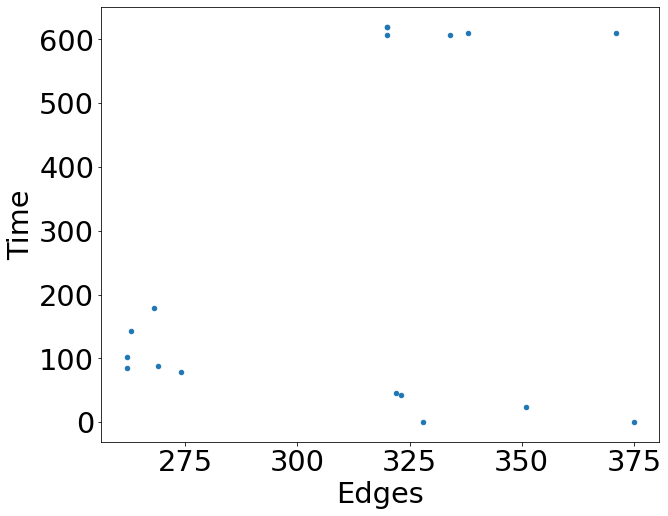
\includegraphics[width=0.95\linewidth]{figures/ssh/edges.png} 
		\caption{Élek} 
		\vspace{4ex}
	\end{subfigure} 
	\begin{subfigure}[b]{0.5\linewidth}
		\centering
		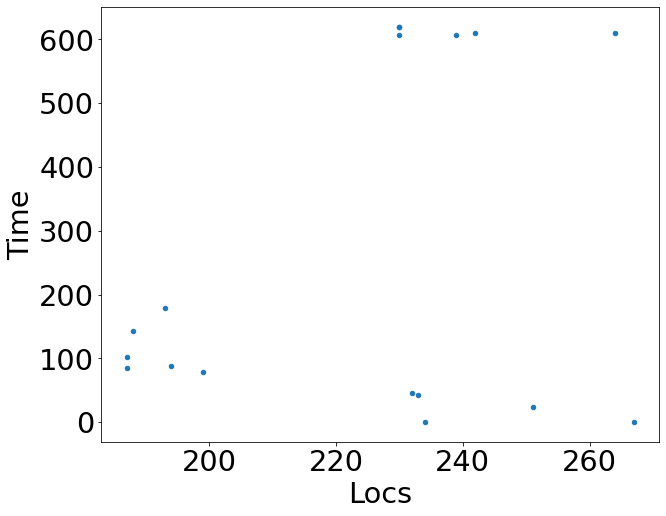
\includegraphics[width=0.95\linewidth]{figures/ssh/locs.png} 
		\caption{Helyek} 
	\end{subfigure}%%
	\begin{subfigure}[b]{0.5\linewidth}
		\centering
		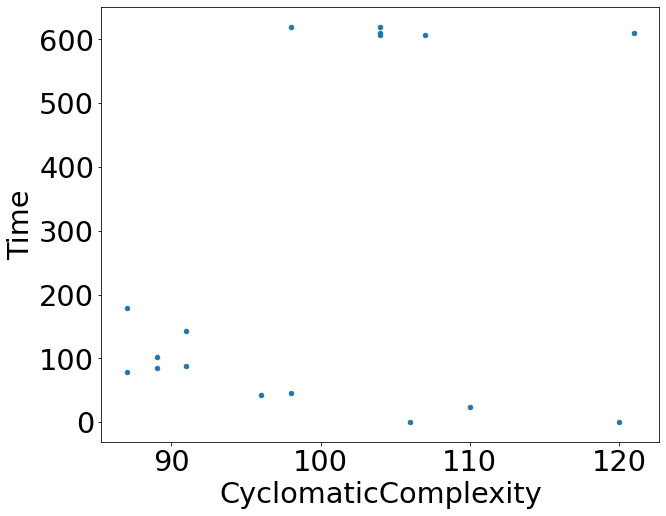
\includegraphics[width=0.95\linewidth]{figures/ssh/cc.png} 
		\caption{Ciklikus komplexitás} 
	\end{subfigure} 
	\caption{SSH tesztkategória.}
	\label{fig_ssh} 
\end{figure}

\begin{figure}[ht] 
	\begin{subfigure}[b]{0.5\linewidth}
		\centering
		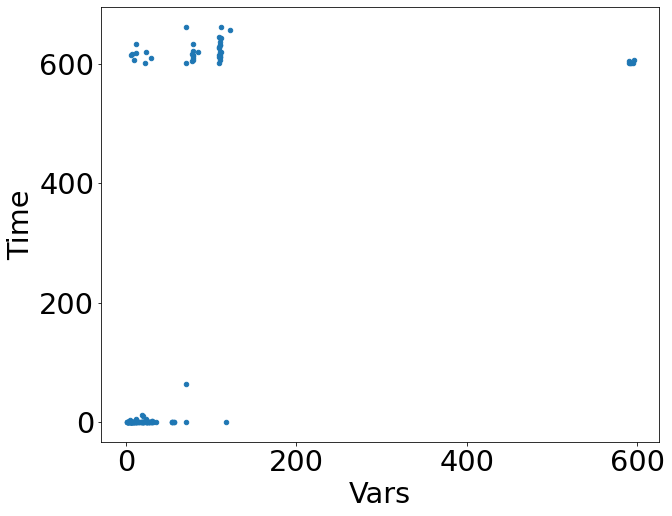
\includegraphics[width=0.95\linewidth]{figures/plc/vars.png} 
		\caption{Változók} 
		\vspace{4ex}
	\end{subfigure}%% 
	\begin{subfigure}[b]{0.5\linewidth}
		\centering
		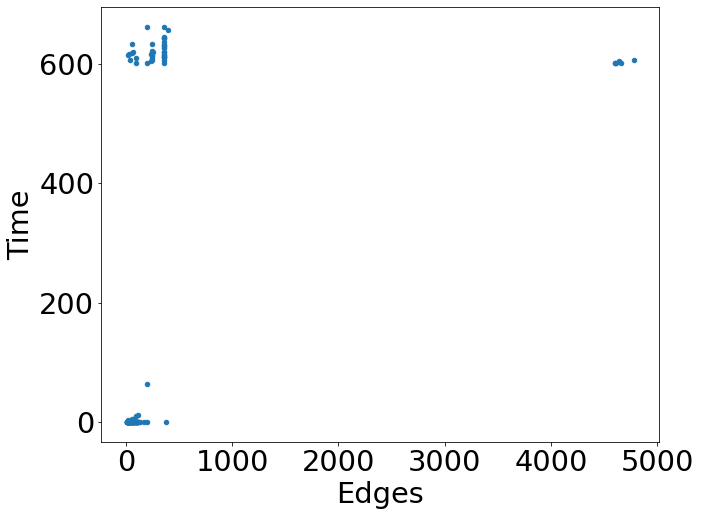
\includegraphics[width=0.95\linewidth]{figures/plc/edges.png} 
		\caption{Élek} 
		\vspace{4ex}
	\end{subfigure} 
	\begin{subfigure}[b]{0.5\linewidth}
		\centering
		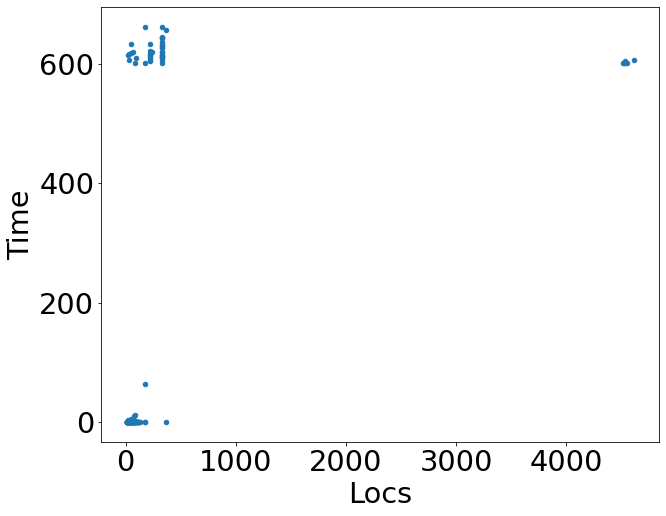
\includegraphics[width=0.95\linewidth]{figures/plc/locs.png} 
		\caption{Helyek} 
	\end{subfigure}%%
	\begin{subfigure}[b]{0.5\linewidth}
		\centering
		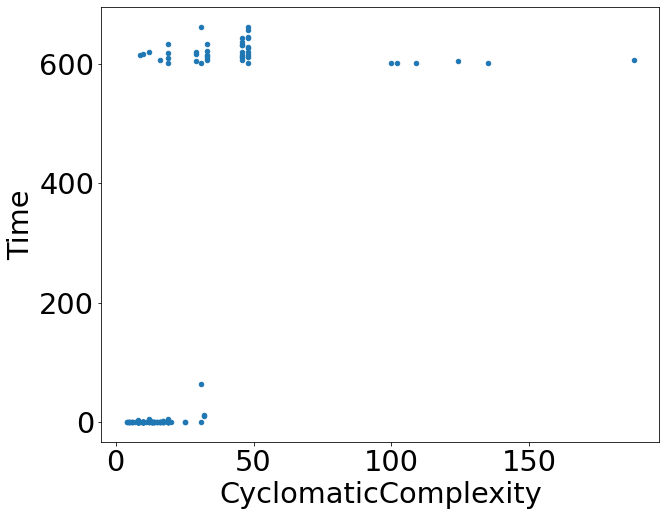
\includegraphics[width=0.95\linewidth]{figures/plc/cc.png}
		\caption{Ciklikus komplexitás}
	\end{subfigure}
	\caption{PLC tesztkategória.}
	\label{fig_plc}
\end{figure}

\begin{figure}[ht] 
	\begin{subfigure}[b]{0.5\linewidth}
		\centering
		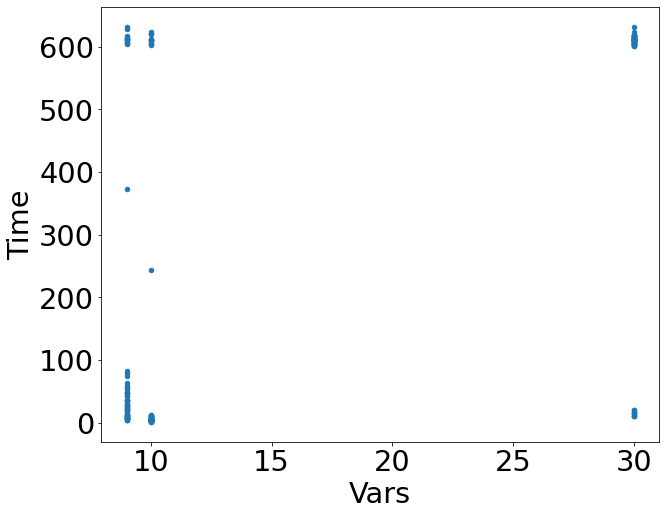
\includegraphics[width=0.95\linewidth]{figures/eca/vars.png} 
		\caption{Változók} 
		\vspace{4ex}
	\end{subfigure}%% 
	\begin{subfigure}[b]{0.5\linewidth}
		\centering
		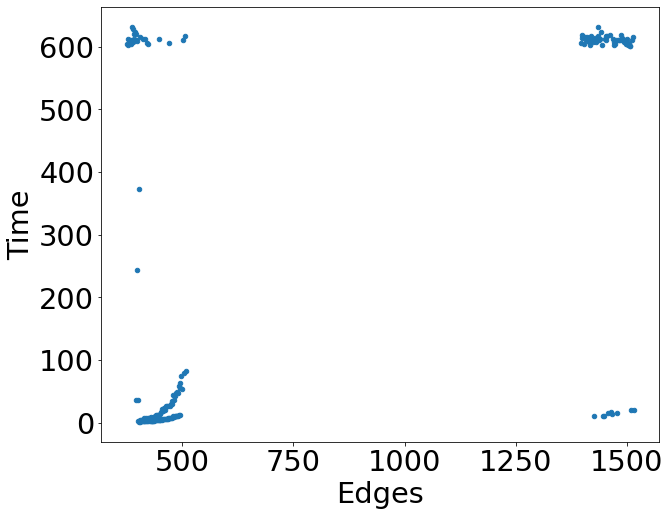
\includegraphics[width=0.95\linewidth]{figures/eca/edges.png} 
		\caption{Élek} 
		\vspace{4ex}
	\end{subfigure} 
	\begin{subfigure}[b]{0.5\linewidth}
		\centering
		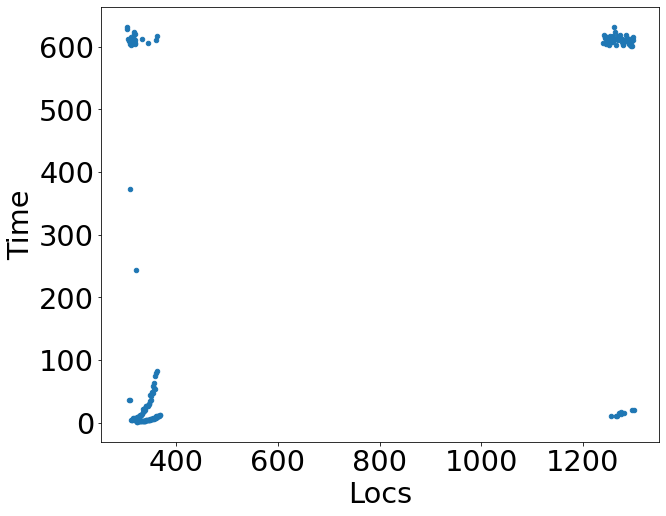
\includegraphics[width=0.95\linewidth]{figures/eca/locs.png} 
		\caption{Helyek} 
	\end{subfigure}%%
	\begin{subfigure}[b]{0.5\linewidth}
		\centering
		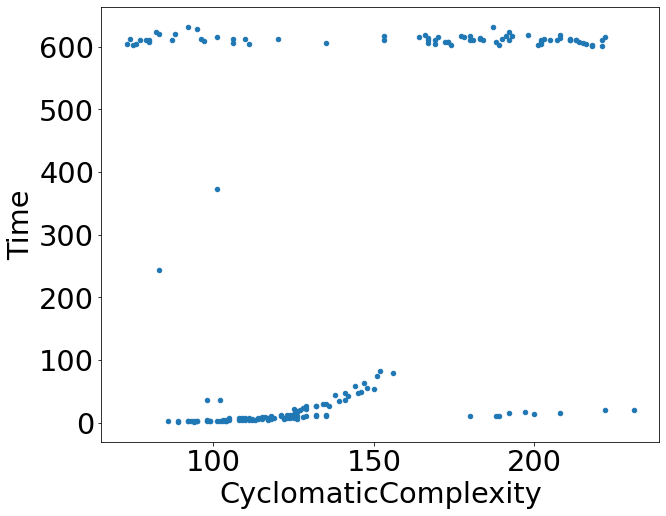
\includegraphics[width=0.95\linewidth]{figures/eca/cc.png} 
		\caption{Ciklikus komplexitás\label{fig_eca_cc} }
	\end{subfigure} 
	\caption{ECA tesztkategória.\label{fig_eca} }
\end{figure}

\clearpage

% --------------------------------------------------------------------------

\section{A parancssori interfész felülete}
\label{sec:parancs_int_fel}

\begin{figure}[!ht]
	\label{fig:cli_1cc}
	\centering
	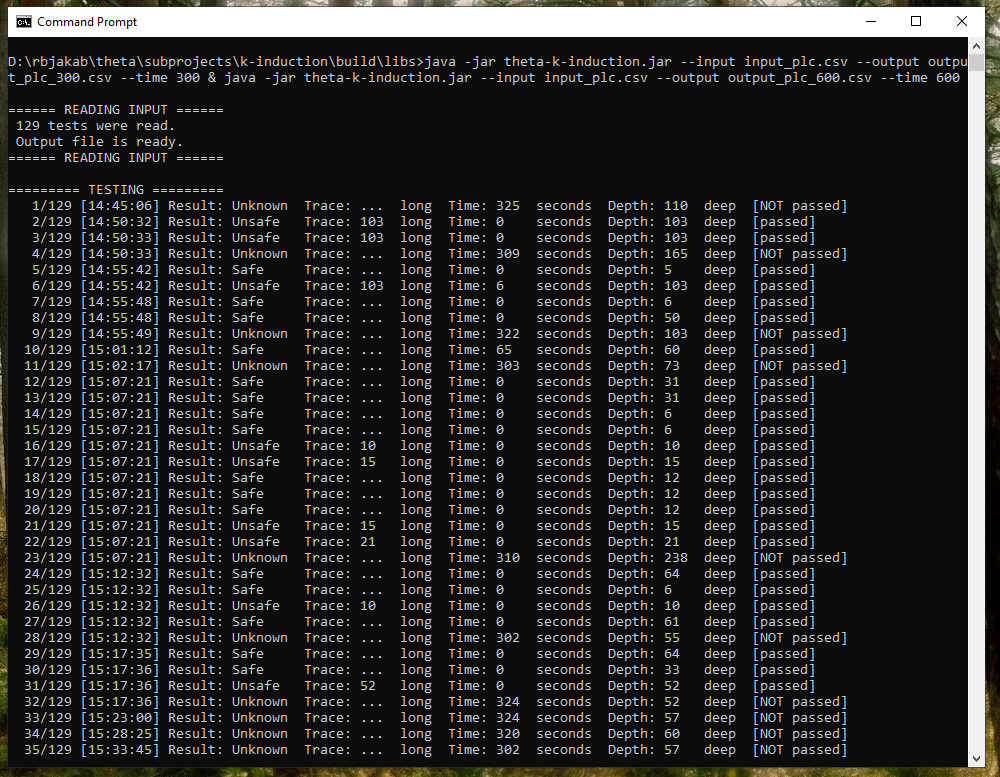
\includegraphics[width=135mm, keepaspectratio]{figures/cli/eleje.png}
	\caption{A parancssori interfész a futás elején.} 
\end{figure}

\begin{figure}[!ht]
	\label{fig:cli_2bb}
	\centering
	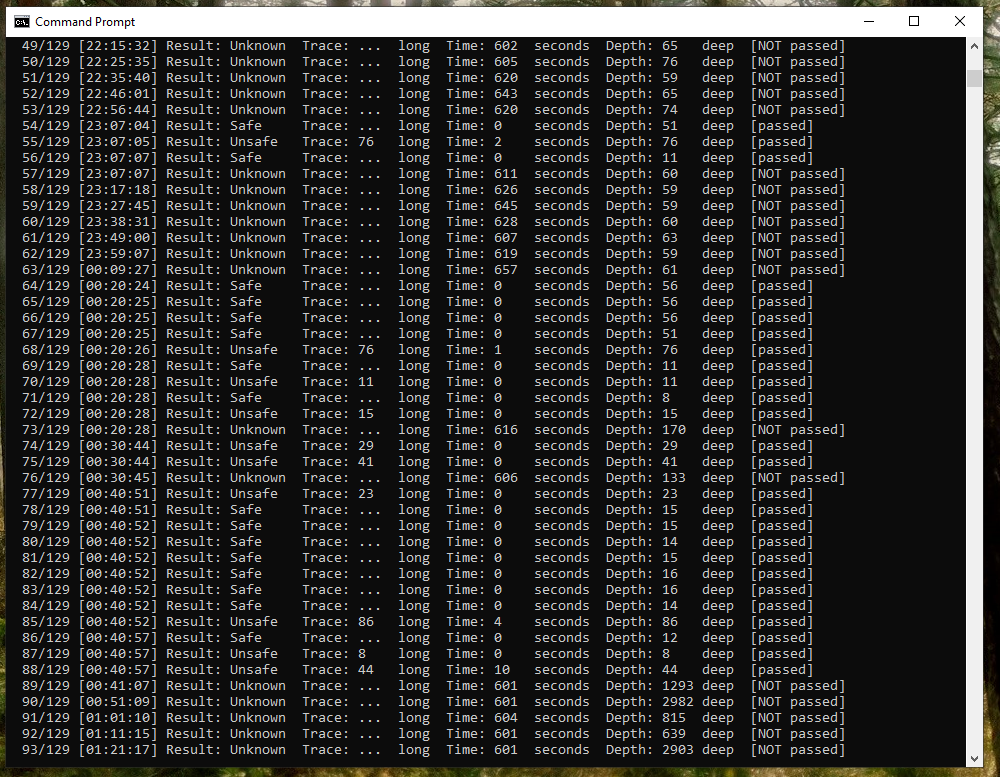
\includegraphics[width=135mm, keepaspectratio]{figures/cli/kozepe.png}
	\caption{A parancssori interfész futás közben.} 
\end{figure}

\begin{figure}[!ht]
	\centering
	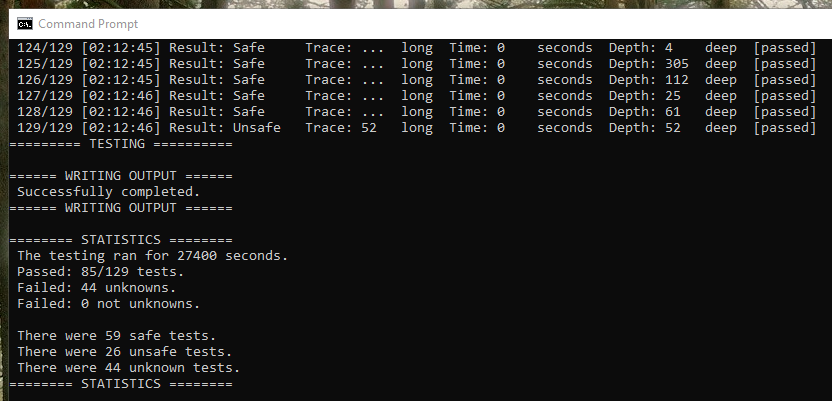
\includegraphics[width=135mm, keepaspectratio]{figures/cli/vege.png}
	\caption{A parancssori interfész a futás végén.\label{fig:cli_3}} 
\end{figure}